\chapter{Einleitung}
Der technologische Fortschritt in der medizinischen Bildgebung hat dazu geführt, dass es heute in der klinischen Diagnostik selbstverständlich ist, innerhalb weniger Minuten den kompletten Patienten  mit hoher Auflösung und hohem Kontrast abzubilden.
Dabei spielt die \gls{mrt} heute nicht nur für die morphologische, sondern auch für die funktionelle oder Diffusions-gewichtete Bildgebung eine entscheidende Rolle. Gegenüber anderen Verfahren, auch \textit{Modalitäten} genannt, bietet die \gls{mrt} zahlreiche Vorteile: Es entstehen Schnittbilder, die mit einem sehr hohen Weichteilkontrast einen (Schatten-freien) Einblick in den Körper liefern. Im Gegensatz zur \gls{ct} kommt dabei keine ionisierende Strahlung zum Einsatz: Statt die Abschwächung von Röntgenstrahlung durch den Körper zu messen, wir der \gls{nmr}-Effekt von Wasserstoffprotonen im Körper genutzt. Durch die verschiedenen möglichen Bildgewichtungen, wie zum Beispiel nach der Protonendichte oder nach der longitudinalen Relaxationszeit und die zahlreichen möglichen Pulssequenzen kann mehr auf den Bildentstehungsprozess als beim Röntgen und bei der \gls{ct}. Dadurch kann oft auf ein Kontrastmittel verzichtet werden.

Die Entwicklungen in der klinischen Bildgebung wirken sich auch positiv auf den Sektor der \textit{präklinischen Bildgebung} (eng. preclinical imaging) aus. Durch die inzwischen möglichen sehr hohen Auflösungen und kurze Aufnahmezeiten ist die Abbildung von Kleintieren, wie Mäusen, Ratten oder anderen Nagern, möglich (vgl. \autoref{fig:fortschritt}). 

\begin{figure}[H]
	\centering
	\subcaptionbox{Eine der ersten MRT-Aufnahmen eines lebendigen Menschens, 1977, \cite{damadian1977}}{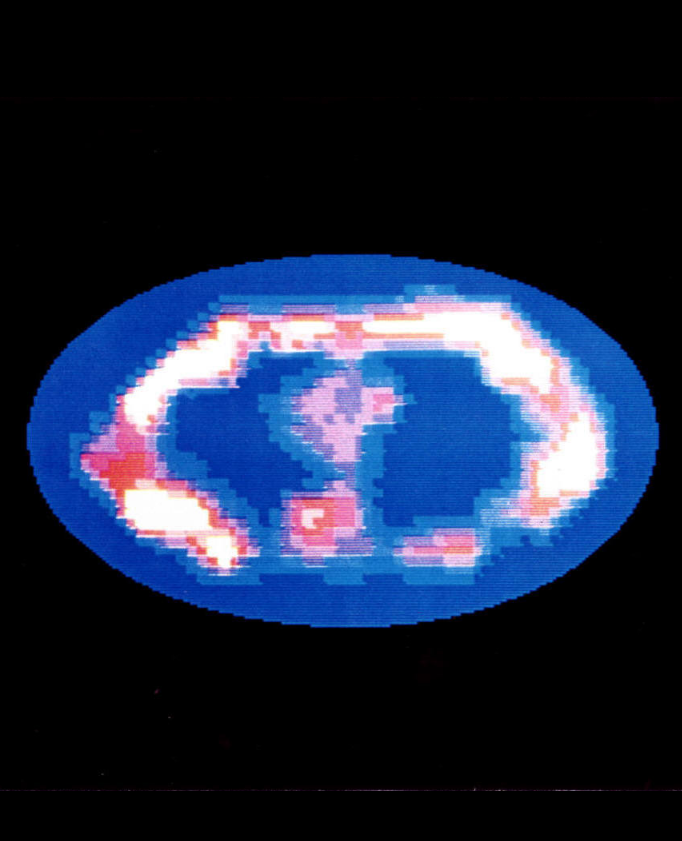
\includegraphics[width=0.45\textwidth]{img/fonarImage.PNG}}
	\hfill
	\subcaptionbox{Hochauflösende MRT-Aufnahme einer Maus, 2013,  \cite{rascheUlm}}{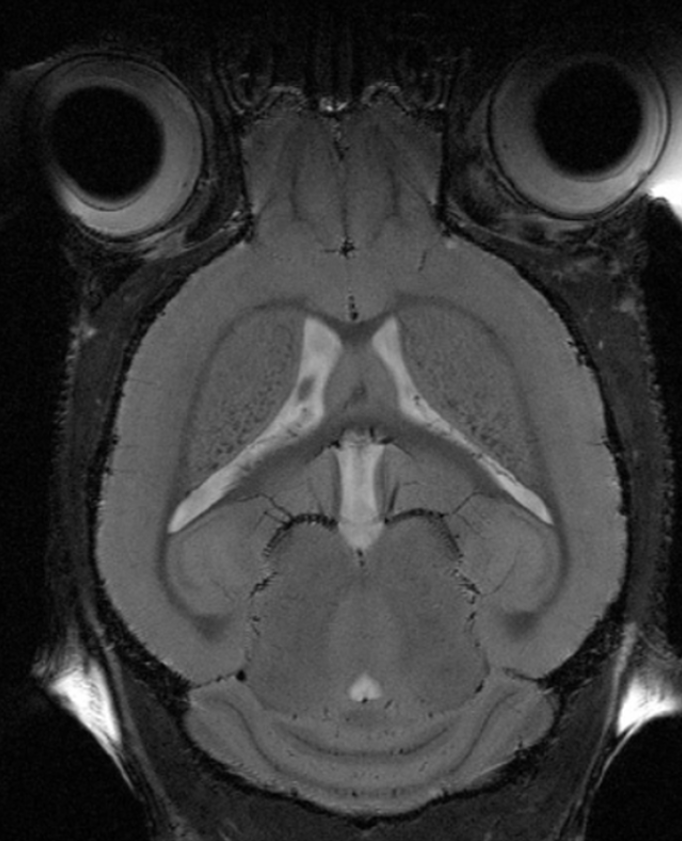
\includegraphics[width=0.45\textwidth]{img/mouseBrain.PNG}}
	\caption{Fortschritt in der MR-Bildgebung 1977 bis 2013}
	\label{fig:fortschritt}
\end{figure}

Bla

 
\section{Ausgangssituation und Aufgabenstellung}
In einer typischen Konfiguration eines Bruker MR-Tomographens werden ein RF-Sendekanal und mehrere RF-Empfangskanäle verwendet. Übliche MRT Prozeduren in der präklinischen Bildgebung nutzen vier oder mehr Empfangsspulen. In der NMR-Spektrometrie wird eine gleiche Anzahl an Sende- und Empfangsspulen eingesetzt.

Aktuell teilen sich die Bruker NMR-Spektrometer der \textit{AVANCE NEO} Generation und MR-Tomographen der \textit{BioSpec}-Linie große Teile der Hochfrequenz-Elektronik. Sende- und Empfangselektronik für die in der Magnetresonanz-Technik notwendigen RF Pulse mit Frequenzen von \SI{40}{\mega\hertz} bis einigen hundert \SI{}{\mega\hertz} sind auf Steckkarten für modulare Chassis-Systeme untergebracht. Dabei besteht eine Steckkarte (TRX1200, siehe \autoref{fig:trx12004er}) immer aus einem Sendepfad mit allen nötigen Wandlern und Verstärkern und einem Empfangspfad mit Eingangsverstärkern und ADCs.

Kommt eine solche Anordnung in der MRT zum Einsatz, ergibt sich eine Situation wie in \autoref{fig:trx12004er} angedeutet: Bei vier notwendigen Karten wird lediglich eine voll ausgenutzt. Bei den restlichen TRX1200 Karten bleibt die Sendeelektronik ungenutzt.

\begin{figure}[H]
	\centering
	\resizebox{0.8\textwidth}{!}{\includegraphics[]{img/trx1200mult.tikz}}
	\caption[Bruker Avance Neo TRX1200 Karte]{AV4 TRX1200 (verwendet in Bruker Avance Neo NMR Spektrometer und einigen MR-Tomographen)}
	\label{fig:trx12004er}
\end{figure}

Für zukünftige Produktentwicklungen sollen vorab in einem Technologieprojekt Möglichkeiten zu Optimierung der Signalkette evaluiert werden. Dabei spielen neben technischen Optimierungsmöglichkeiten auch wirtschaftliche Aspekte eine Rolle.
Durch die unterschiedlichen Qualitätsanforderungen an die der Sende- und Empfangselektroniken in der NMR und der MRT ergibt sich ein Einsparpotential: Da in der NMR Spektren über die Fouriertransformation des FID gemessen werden, ist zum Erreichen einer hohen spektralen Auflösung aufgrund der Reziprozität von Zeit- zu Frequenzbereich eine lange Messzeit\footnote{Bis hin zu mehreren Stunden} notwendig. An das Taktsignal des, zur Digitalisierung des FIDs, genutzten ADC werden daher hohe Stabilitätsanforderungen gestellt. In der MRT dauert die Aufnahme eines Empfangssignals (in der Regel kein FID, sondern ein Echo) meist nur wenige Millisekunden. Die Zeitdauern sind bei der klassischen MRT zur morphologischen Bildgebung durch die verschiedenen eingesetzten Pulssequenzen, die gewünschte Ortsauflösung, etc. bestimmt.
Durch die kürzere Akquisitionszeit einer MRT-Aufnahme im Vergleich zu einem NMR-Spektrum werden weniger strenge Anforderungen bezüglich der zeitlichen Langzeitstabilität an den Referenzoszillator gestellt.

Zur Charakterisierung der Einflüsse eines weniger stabilen Oszillators und anderer potenziell negativer Einflüsse auf die MR-Signale soll eine Simulation eingesetzt werden. Statt die komplette Signalkette auf der Ebene der einzelnen elektronischen Baugruppen durchzurechnen wird zunächst auf einer höheren Abstraktionsebene angesetzt. In einer Simulation beginnend von einer dreidimensionalen Eingangsmatrix werden Schichtbilder simuliert, wie sie auch ein MR-Tomograph erzeugen würde. Dazu müssen die Vorgänge, wie sie im echten Gerät ablaufen, nur in soweit modelliert werden, wie sie für die zu untersuchende Störung relevant sind. Da in dieser Arbeit der Einfluss von Phasenrauschen des Referenzoszillators und damit des ADC-Taktsignals in Abhängigkeit verschiedener MRT-Pulssequenzen untersucht werden soll, ist es für die Simulation erforderlich, verschiedene Pulssequenzen abfahren zu können und das RF-Empfangssignal gezielt zu manipulieren.

Für numerische Simulationen in den Natur- und Ingenieurwissenschaften ist das Programmpaket \textit{MATLAB}\cite{matlab} von \textit{The MathWorks} weit verbreitet. Es existieren einige Ver\-öffent\-lichungen zu MRT-Simulationen in MATLAB\footnote{zum Beispiel \cite{Kern2012}}, in denen sich die Autoren meist auf die Simulation bestimmter Teilaspekte der MRT beschränken. Mehr auf eine vollständige Simulation ausgerichtet ist das Programm \textit{MRiLab}\cite{Liu2017} (siehe \autoref{fig:mrilabscreenshot}).


In dieser Arbeit soll MRiLab auf die Eignung als Simulationsumgebung für kommende Entwicklungstätigkeiten bei Bruker BioSpin hin untersucht werden.


